\chapter{数值模型建立与验证}\label{chap:model}

\section{物理问题描述与几何模型}

\subsection{打印系统几何构型}

本论文的研究对象为一种带有整形板结构的挤出式三维混凝土打印（3D Concrete Printing, 3DCP）喷嘴组合体，其整体结构主要由喷嘴主体与后置整形板两部分组成。该结构旨在模拟打印混凝土在实际挤出沉积过程中的流动、压实与成形行为，并研究不同几何参数对打印质量与流场特性的影响规律。

喷嘴主体由竖直圆柱形入口直管、锥形收缩段以及出口直管段组成。喷嘴入口直管长度（Straight Tube Length）为100~mm，用于保证浆体在进入收缩区域前形成相对稳定的流动状态。锥形收缩段（竖向长度L、半锥角$\theta$）对混凝土浆体进行渐缩加压，使流体由较大截面逐渐过渡至出口区域，进一步稳定出口流场并控制挤出过程中的速度分布。

整形板结构安装于喷嘴出口下方，主要由顶部水平板、前挡板、左右侧板以及倾斜出料段组成。左右侧板厚度均为11~mm，用于限制打印材料横向扩散。整形板倾斜出料段长度记为TL，倾角记为$\alpha$。整形板的主要功能是在混凝土挤出后对其进行二次压实与几何整形，以改善打印层的表面平整度、层间接触质量以及截面一致性。喷嘴出口底面与基底面之间的垂直距离定义为$Z_0$。本研究中限制$Z_0 = 22$~mm，以保证混凝土打印层高的可用性与CFD建模结果的可对比性。

打印过程中，混凝土材料经喷嘴挤出后，其最终形成的打印层高度$H$不仅受到喷嘴出口高度的影响，还与整形板倾斜出料段的几何参数密切相关。根据几何关系，打印层高度可表示为：
\begin{equation}\label{eq:H}
  H = Z_0 - TL \cdot \sin(\alpha).
\end{equation}
由此进一步可得打印层高度对倾角$\alpha$的偏导关系为：
\begin{equation}\label{eq:dH-dalpha}
  \frac{\partial H}{\partial \alpha} = -TL \cos(\alpha) < 0.
\end{equation}
由\cref{eq:dH-dalpha}可知，在TL保持不变的条件下，随着整形板倾角$\alpha$增大，打印层高度$H$将逐渐减小，即整形板对材料的压实作用增强。这表明整形板几何参数会直接影响打印层的压实程度与沉积形态，是本课题的研究重点之一。

考虑到实际3D打印混凝土施工中，不同打印对象对于层高具有不同要求，本研究参考现有打印工艺范围，将打印层高度的研究边界设定为：
\begin{equation}\label{eq:H-range}
  5~\text{mm} \leq H \leq 20~\text{mm}.
\end{equation}
该范围能够覆盖大多数挤出式混凝土打印的典型层高条件，同时兼顾打印稳定性与结构成形质量。

组合体几何模型的三维结构示意图以及主要几何参数定义的侧视剖面图分别如\cref{fig:2.1}与\cref{fig:2.2}所示。

\begin{figure}[!htb]
  \centering
  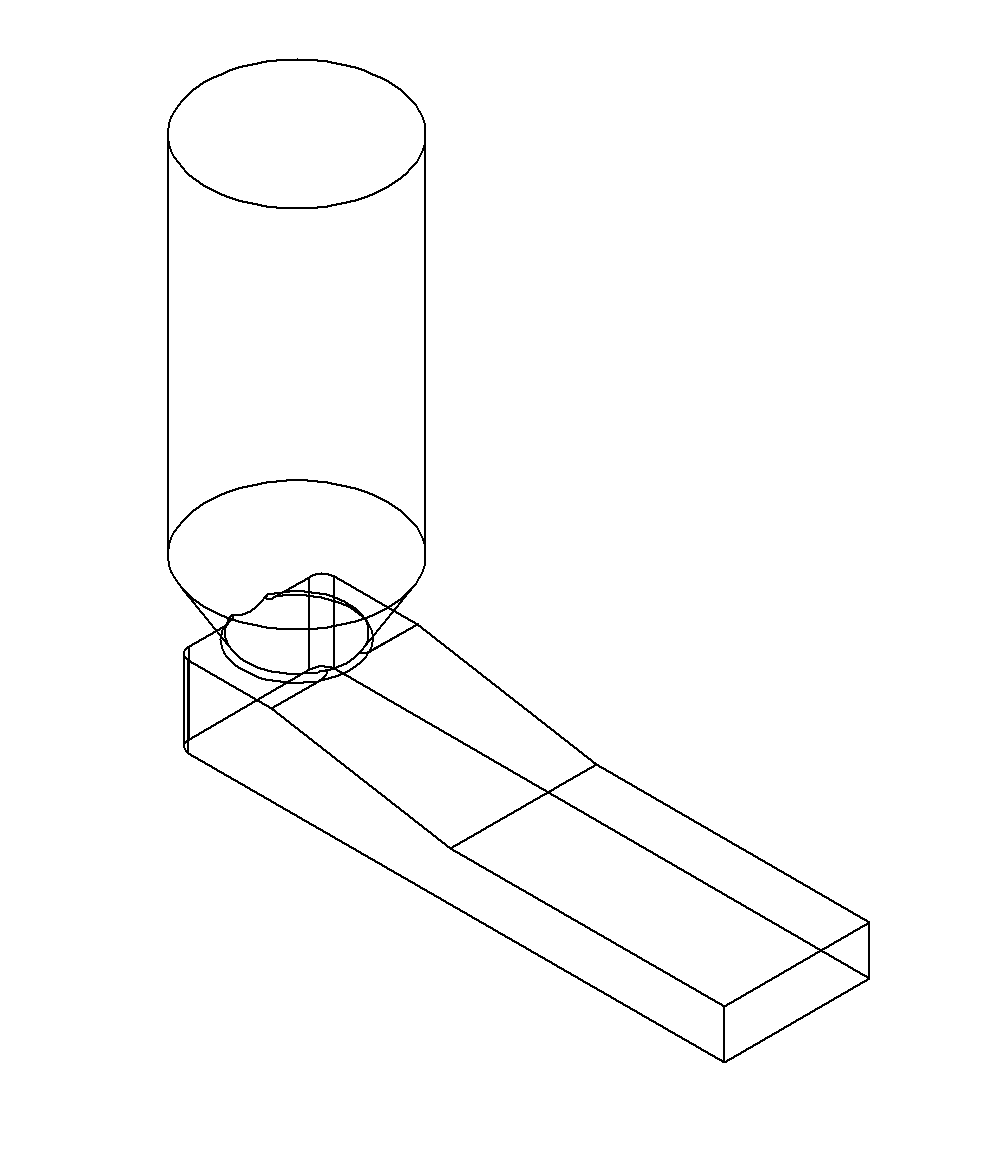
\includegraphics[width=0.7\textwidth]{figures/2.1.PNG}
  \caption{几何模型三维示意图}
  \label{fig:2.1}
\end{figure}

\begin{figure}[!htb]
  \centering
  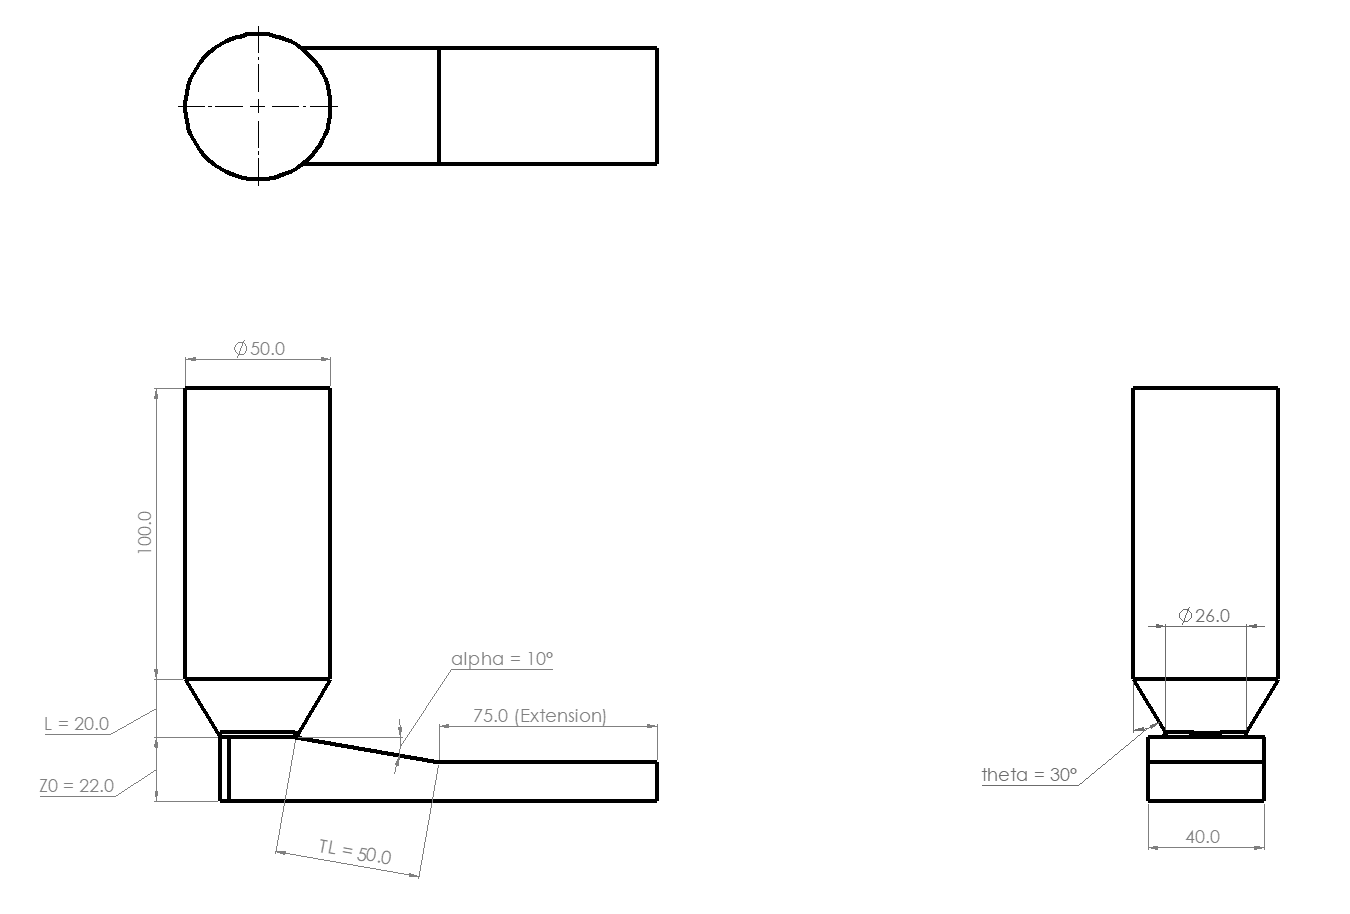
\includegraphics[width=0.7\textwidth]{figures/2.2.png}
  \caption{几何参数定义侧视剖面图}
  \label{fig:2.2}
\end{figure}

为研究喷嘴与整形板结构参数对打印流场及成形性能的影响规律，本文选取四个关键几何参数作为主要研究变量：锥形收缩段半锥角$\theta$、喷嘴竖直长度L、整形板倾斜出料段长度TL以及倾斜角$\alpha$。研究重点分析上述参数对基底接触压力（Substrate Pressure）、剪切应力（Shear Stress）以及压力传递效率（Pressure Transfer Efficiency）等指标的影响机制。除上述变量外，其余结构参数均采用He等\cite{he2024}中所提出的标准尺寸，以保证模型具有一定的工程参考价值与对比一致性。

各参数组合与对应工况汇总如\cref{tab:2.1}所示。

\begin{table}[!htb]
  \centering
  \caption{几何参数定义与基准值汇总}\label{tab:2.1}
  \renewcommand{\arraystretch}{1.3}
  \begin{tabular}{cclc}
    \toprule
    \textbf{参数} & \textbf{符号} & \textbf{基准值} & \textbf{变化范围} \\
    \midrule
    入口直径   & $D_{in}$  & 47 mm & 固定（由$\theta$、L、$D_{out}$决定） \\
    出口直径   & $D_{out}$ & 26 mm & 固定 \\
    收缩角     & $\theta$  & 30°   & 0°, 15°, 30°, 45°, 60° \\
    直管段长   & $L$       & 20 mm & 10, 20, 30, 40 mm \\
    整形板长   & $TL$      & 50 mm & 30, 40, 50, 55, 60, 70 mm \\
    倾斜角     & $\alpha$  & 10°   & 0°, 5°, 10°, 15°, 20° \\
    出口距基底 & $Z_0$     & 22 mm & 固定 \\
    侧板/前板厚 & $t$      & 11 mm & 固定 \\
    \bottomrule
  \end{tabular}
\end{table}

\subsection{坐标系与边界面定义}

为便于对打印混凝土在喷嘴及整形板内部的流动行为进行分析，并统一后续压力、速度及剪切应力等物理量的方向定义，本课题建立三维直角坐标系对计算域进行描述。其中，Y轴定义为竖直方向，正方向向上；X轴定义为打印方向，即混凝土材料沿整形板延伸方向的运动方向；Z轴定义为横向方向，用于描述打印层宽度方向上的流动特征。重力加速度$g$沿Y轴负方向施加，其取值为：
\begin{equation}\label{eq:gravity}
  g = -9.81~\text{m/s}^2,
\end{equation}
用于模拟实际打印过程中混凝土浆体在自重作用下的流动与沉积行为。

为定量分析流场内部不同区域的流动特征，本课题在模型中设置了多个监测边界面与特征截面，以便后续提取压力、速度、剪切应力及质量流量等关键参数。各边界面定义如下：

（1）Inlet（喷嘴入口顶面）：Inlet为喷嘴入口顶面，其法向方向垂直于Y轴，用于施加入口边界条件，包括入口速度、体积流量及材料流变参数等。

（2）Nozzle Outlet Plane（喷嘴出口截面）：Nozzle Outlet Plane为喷嘴出口截面，其法向方向同样垂直于Y轴。该截面用于分析混凝土材料在离开喷嘴瞬间的速度分布、静压力分布及流场均匀性，是研究喷嘴内部压力传递行为的重要监测位置。

（3）Trowel Outlet Plane（出料口截面）：Trowel Outlet Plane为整形板倾斜出料段末端截面，其法向方向垂直于X轴。该截面主要用于研究整形板对材料流动状态及截面形状的整形作用，并用于评估挤出后材料的速度稳定性与压实效果。

（4）Outlet（延伸段边界面）：Outlet为计算域末端延伸段出口边界，其法向方向垂直于X轴。该边界用于保证流场出口区域具有充分发展长度，从而减小出口边界条件对主流场计算结果的影响。

（5）Substrate（打印基底面）：Substrate为打印基底面，其平面方向平行于XZ平面，用于模拟实际打印过程中的基板接触界面。该区域是研究基底接触压力、剪切应力以及层间压实行为的关键监测区域。

（6）Wall（外部壁面）：Wall是所有在混凝土挤出过程中对流体施加空间边界条件的面，由喷嘴直管壁面、喷嘴收缩段壁面、整形板上顶面、整形板前、左、右壁面共同组成。

上述边界面的空间位置关系如\cref{fig:2.3}所示。

\begin{figure}[!htb]
  \centering
  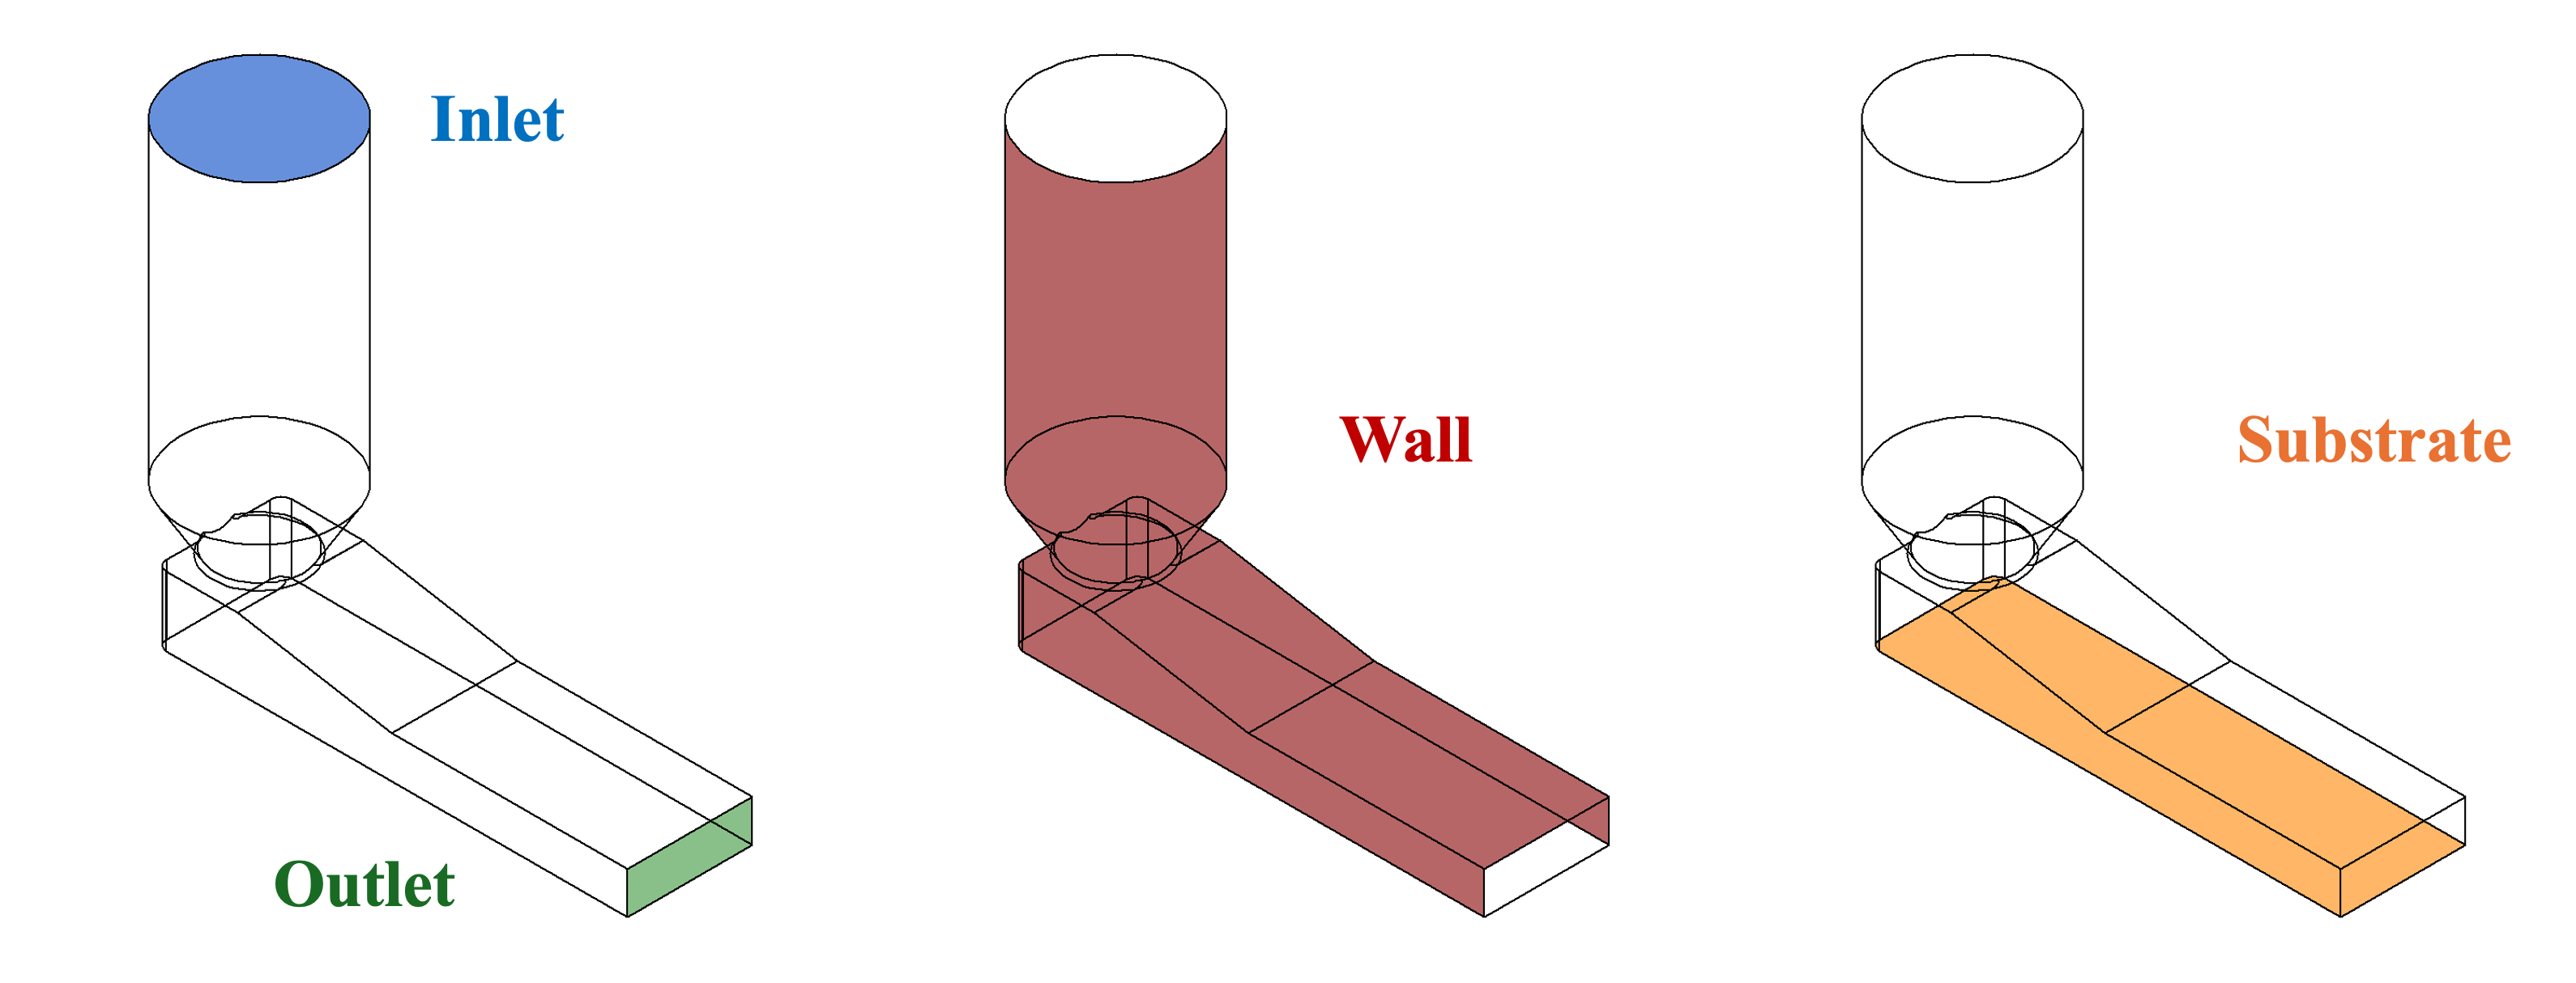
\includegraphics[width=0.7\textwidth]{figures/2.3.png}
  \caption{边界条件分布示意图}
  \label{fig:2.3}
\end{figure}

\section{控制方程与本构模型}

\subsection{连续方程与动量方程}

为描述打印混凝土浆体在喷嘴内部及整形板区域的流动行为，本文基于计算流体动力学（CFD）建立控制方程。考虑到打印过程中温度变化较小，且浆体流动速度较低，本文将打印混凝土浆体假设为等温、单相、不可压缩稳态非牛顿流体，并忽略材料离析及气泡对流场的影响。

在上述假设条件下，浆体流动满足质量守恒方程与动量守恒方程。不可压缩流体的连续性方程表示为：
\begin{equation}\label{eq:continuity}
  \nabla \cdot \mathbf{u} = 0,
\end{equation}
其中，$\mathbf{u}$是速度矢量。

浆体流动的动量守恒方程采用Navier--Stokes方程表示：
\begin{equation}\label{eq:NS}
  \rho (\mathbf{u} \cdot \nabla) \mathbf{u} = -\nabla p + \nabla \cdot \left[ \eta(\dot{\gamma}) \cdot (\nabla \mathbf{u} + (\nabla \mathbf{u})^T) \right] + \rho \mathbf{g},
\end{equation}
其中，$\rho$为浆体密度（2100~kg/m³），$p$为静压力，$\eta$为黏性应力张量，$\mathbf{g}$为重力加速度矢量（$\mathbf{g} = -9.81 \hat{\mathbf{j}}$~m/s²）；$\eta(\dot{\gamma})$为依赖于局部剪切速率$\dot{\gamma}$的表观黏度，由Herschel--Bulkley本构模型描述。由于打印混凝土浆体在喷嘴内的广义雷诺数$Re_{gen} \approx 0.007 \ll 1$，对流惯性项$\rho(\mathbf{u} \cdot \nabla)\mathbf{u}$远小于黏性项，流动处于蠕动流（Stokes flow）范畴，黏性力主导流场行为。

\subsection{Herschel-Bulkley本构模型}

为更加准确地描述打印混凝土浆体的非牛顿流变特性，本课题采用Herschel-Bulkley（H-B）本构模型对浆体的黏塑性行为进行表征，而未采用传统Bingham模型。相比于Bingham模型，H-B模型能够同时反映材料的屈服应力特性以及剪切变稀行为，更适用于打印混凝土在挤出过程中的复杂流动状态。

Herschel-Bulkley本构模型表示为：
\begin{equation}\label{eq:HB}
  \eta(\dot{\gamma}) = \begin{cases}
    \dfrac{\tau_0}{\dot{\gamma}} + k \dot{\gamma}^{n-1}, & \dot{\gamma} > \dot{\gamma}_c, \\[6pt]
    \dfrac{\tau_0}{\dot{\gamma}_c} + k \dot{\gamma}^{n-1}, & \dot{\gamma} \leq \dot{\gamma}_c,
  \end{cases}
\end{equation}
式中，$\tau_0$为屈服应力（Pa），表征材料开始流动所需克服的最小剪切应力；$k$为稠度系数（$\text{Pa} \cdot \text{s}^n$），反映材料整体黏度水平；$n$为流动指数（无量纲），当$n < 1$时材料表现为剪切变稀行为，当$n = 1$时H-B模型退化为Bingham模型；$\dot{\gamma}_c$为截断剪切速率。H-B模型在低剪切速率区域可能出现表观黏度趋于无穷大的数值问题，$\dot{\gamma}_c$的引入对模型进行Papanastasiou正则化，可提高数值计算稳定性，也可以有效避免低剪切速率区域黏度奇异性。

本文所用各流变参数取值参考已有文献中典型打印混凝土的测量结果，具体见\cref{tab:2.2}。模型对应的黏度-剪切速率关系曲线如\cref{fig:2.4}所示。

\begin{table}[!htb]
  \centering
  \caption{H-B流变参数取值及文献依据}\label{tab:2.2}
  \renewcommand{\arraystretch}{1.3}
  \begin{tabular}{clcl}
    \toprule
    \textbf{参数} & \textbf{符号} & \textbf{取值} & \textbf{物理意义与文献依据} \\
    \midrule
    屈服应力      & $\tau_0$         & 500 Pa            & 材料静止承载能力；参考He\cite{he2024}, Chen\cite{chen2020} \\
    稠度系数      & $k$              & 15 Pa·sⁿ          & 整体黏度水平 \\
    流动指数      & $n$              & 0.45              & 剪切变稀程度（$n<1$）；参考文献取值范围0.3-0.6 \\
    截断剪切速率  & $\dot{\gamma}_c$ & 0.01 s⁻¹          & Papanastasiou正则化截断点 \\
    最大黏度      & $\eta_{max}$     & 50000 Pa·s        & 未屈服区上限 \\
    最小黏度      & $\eta_{min}$     & 1 Pa·s            & 数值稳定下限 \\
    材料密度      & $\rho$           & 2100 kg/m³        & 典型水泥砂浆密度 \\
    \bottomrule
  \end{tabular}
\end{table}

\begin{figure}[!htb]
  \centering
  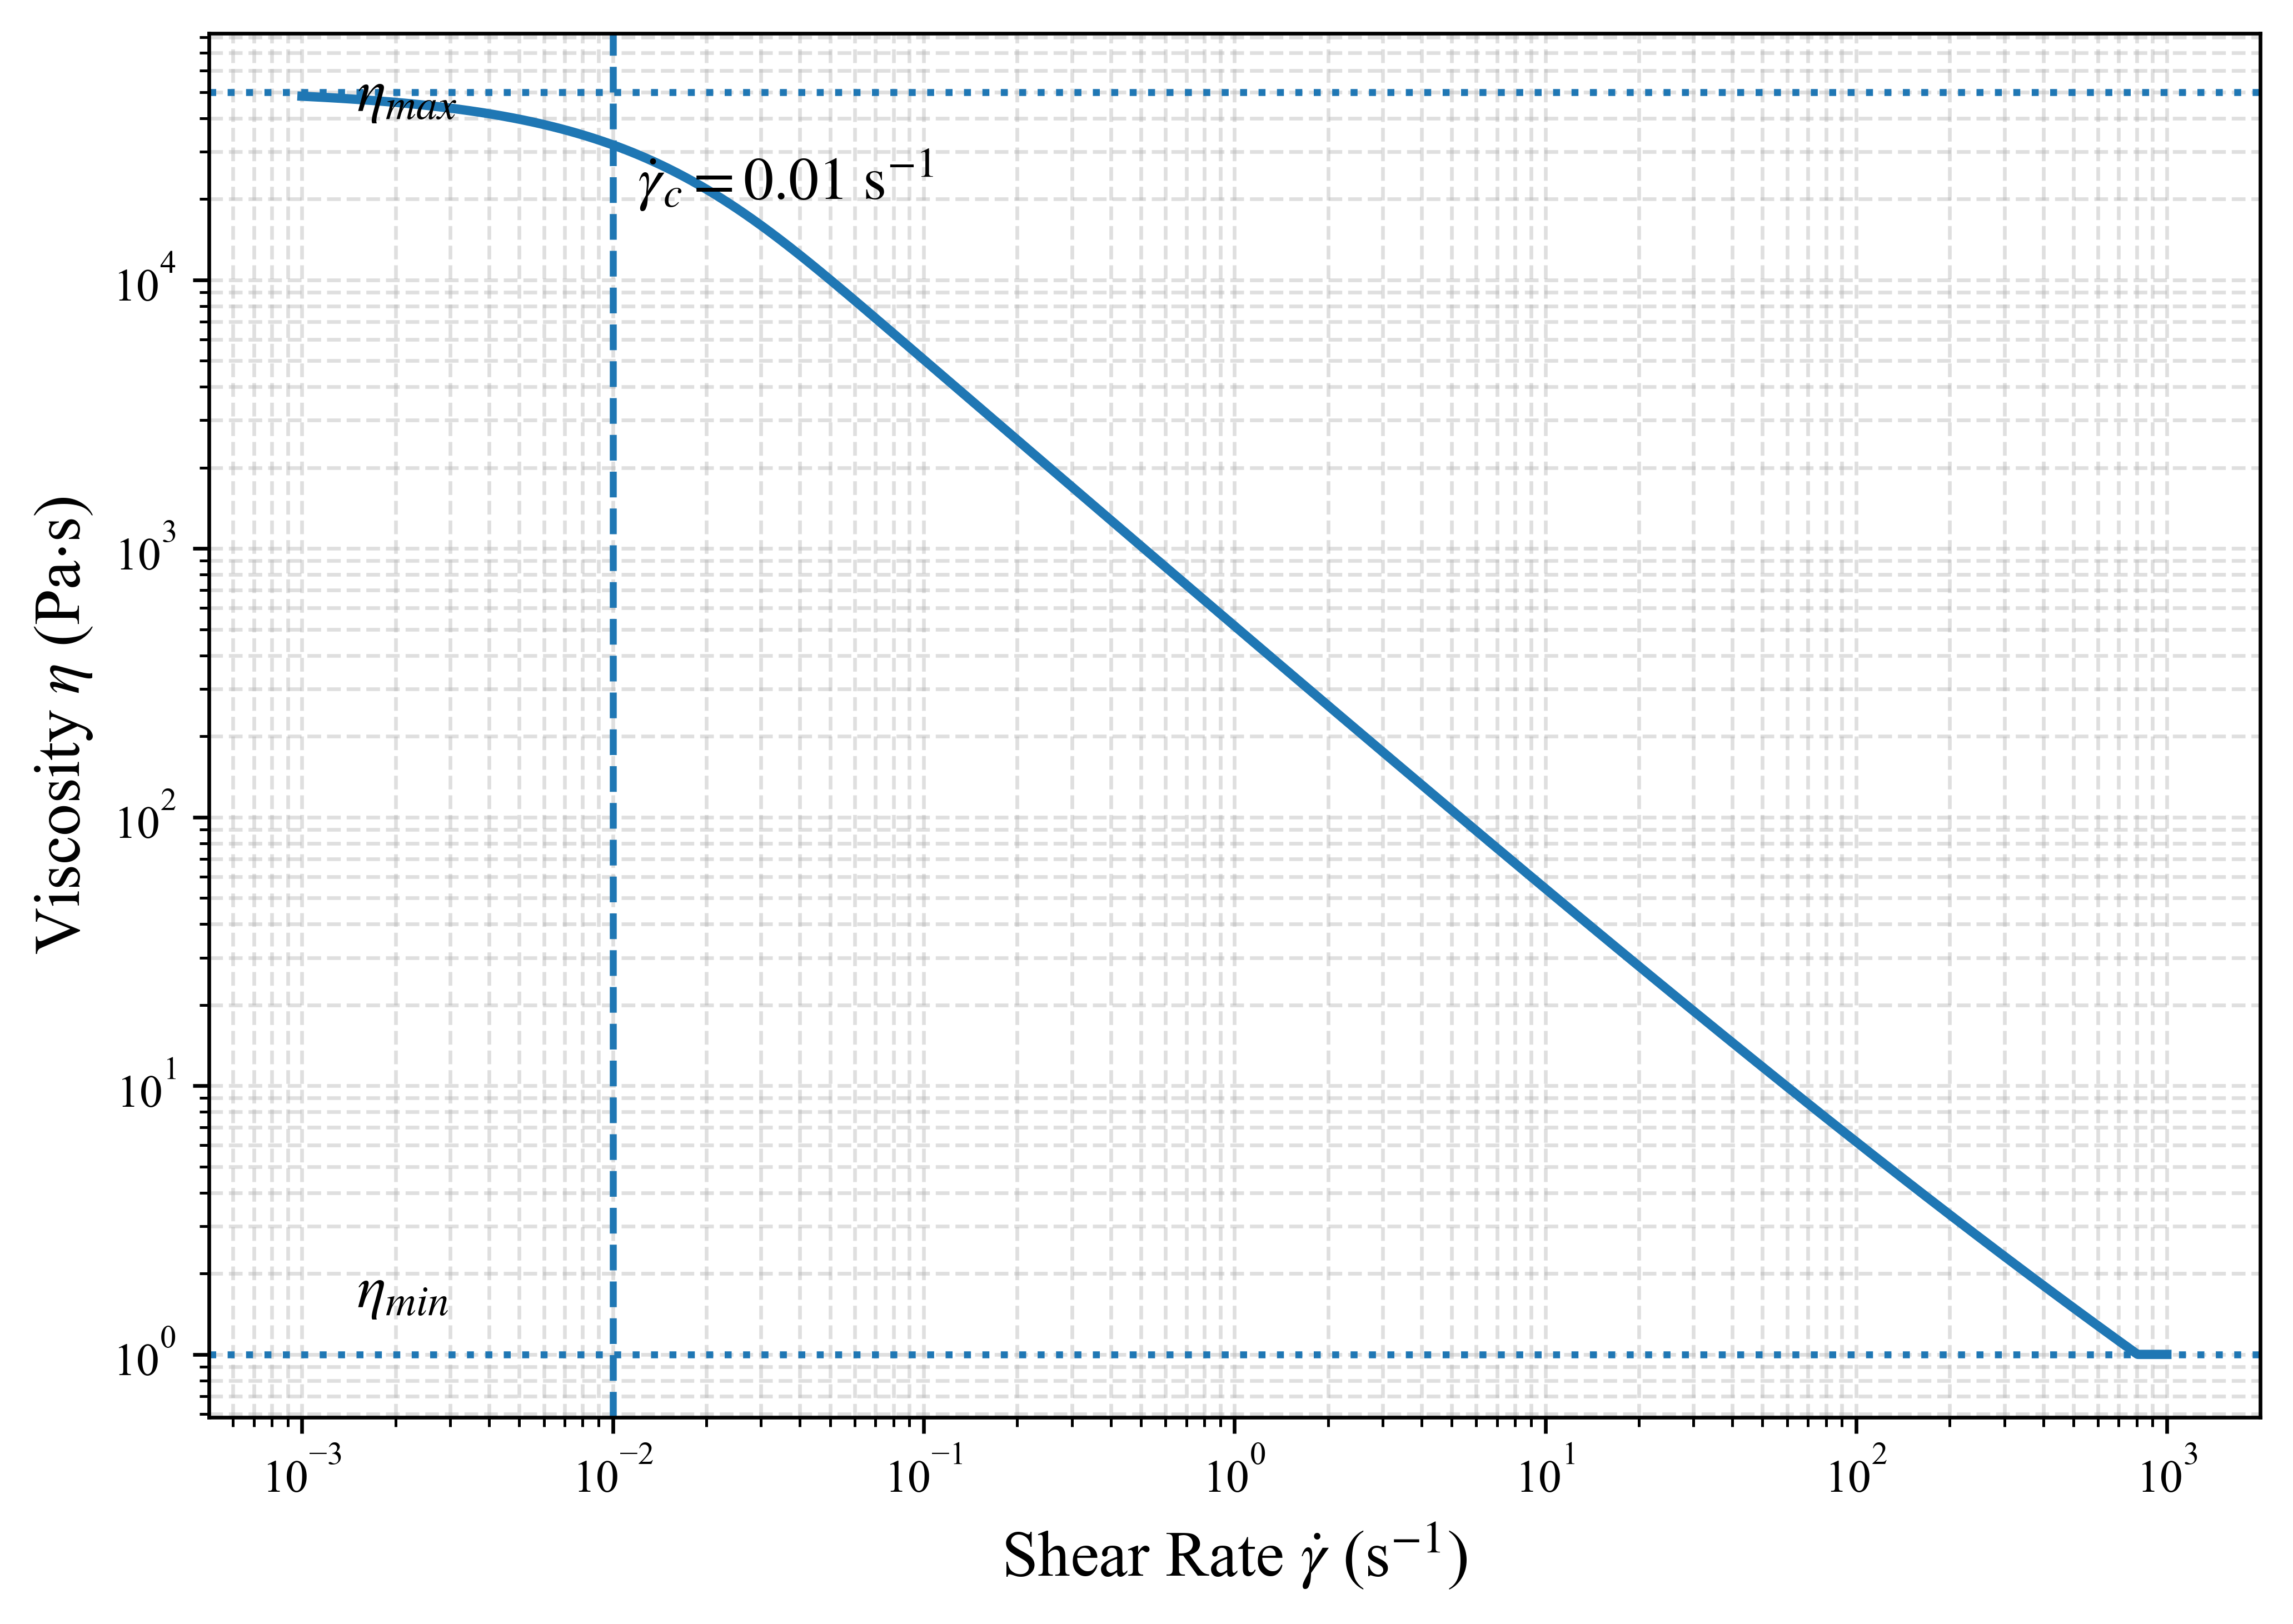
\includegraphics[width=0.7\textwidth]{figures/2.4.png}
  \caption{H-B模型黏度--剪切速率曲线}
  \label{fig:2.4}
\end{figure}

\subsection{雷诺数估算与层流假设验证}

在基准工况（见\cref{chap:baseline}第\ref{sec:baseline-params}节）下，喷嘴出口处典型剪切速率为：
\begin{equation}\label{eq:gamma-typ}
  \dot{\gamma} \approx \frac{v_{in}}{R} \approx \frac{0.03}{0.013} \approx 2.3~\text{s}^{-1}.
\end{equation}
对应有效黏度为：
\begin{equation}\label{eq:eta-eff}
  \eta_{eff} \approx \frac{\tau_0}{\dot{\gamma}} + k \cdot \dot{\gamma}^{n-1} = \frac{500}{2.3} + 15 \times 2.3^{-0.55} \approx 227~\text{Pa} \cdot \text{s}.
\end{equation}
广义雷诺数为：
\begin{equation}\label{eq:Re}
  Re_{general} = \frac{\rho v D}{\eta_{eff}} = \frac{2100 \times 0.03 \times 0.026}{227} \approx 0.0072 \ll 1.
\end{equation}
由以上计算可见，混凝土浆体的广义雷诺数$Re_{general}$远小于1，证明层流假设成立。

\section{计算域离散与网格划分}

\subsection{几何建模与流体域提取}

本课题采用SolidWorks 2024软件建立喷嘴组合体三维几何模型。为实现不同工况下几何参数的快速调整与批量建模，模型构建过程中采用Equation参数化驱动方式，对各草图（Sketch）的关键尺寸进行统一控制，从而实现喷嘴半锥角$\theta$、出口直管长度$L$、整形板长度$TL$及倾角$\alpha$等参数的参数化建模。

完成实体建模后，采用Cavity命令提取组合体内部流体域，以构建后续CFD计算所需的流体计算区域。为提高数值计算稳定性并减小边界条件对主流场的影响，本课题进一步对流体域进行了两部分延伸处理：

（1）在整形板出料口末端沿材料挤出方向增加75~mm自由延伸段，用于模拟浆体离开整形板后的自由流动区域；

（2）保留整形板底部至打印基底面之间的悬空区域，用于描述浆体与基底接触前后的流动与压实行为。

最终建立的流体域主要包括喷嘴入口直管段、锥形收缩段、出口直管段、整形板受限流动区域（由顶部板与侧板围成）以及自由延伸段。

流体域模型导出后，在ANSYS SpaceClaim中对各边界面按照计算规则进行命名，并对几何体封闭性与拓扑连续性进行检查，以保证后续网格划分与数值计算的正确性。

\subsection{网格策略}

本研究采用非结构化四面体网格对流体域进行离散化处理，以平衡计算效率与几何适应性。全局尺寸定义为每个流体域推荐的网格尺寸，以避免对模型的过度复杂化。

为精确捕捉关键区域的流动细节，对喷嘴入口、整形板出口及其接触的圆弧面实施了边缘局部加密策略，确保相关边缘网格尺寸细化至0.5~mm-1~mm。同时，在所有固壁面设置了包含5层单元、增长比为1.2的Inflation边界层，以保障近壁面流动的解析精度。\cref{fig:2.5}与\cref{fig:2.6}分别展示了基础工况的整体网格示意图及喷嘴收缩段与整形板受限区的局部加密细节。

\begin{figure}[!htb]
  \centering
  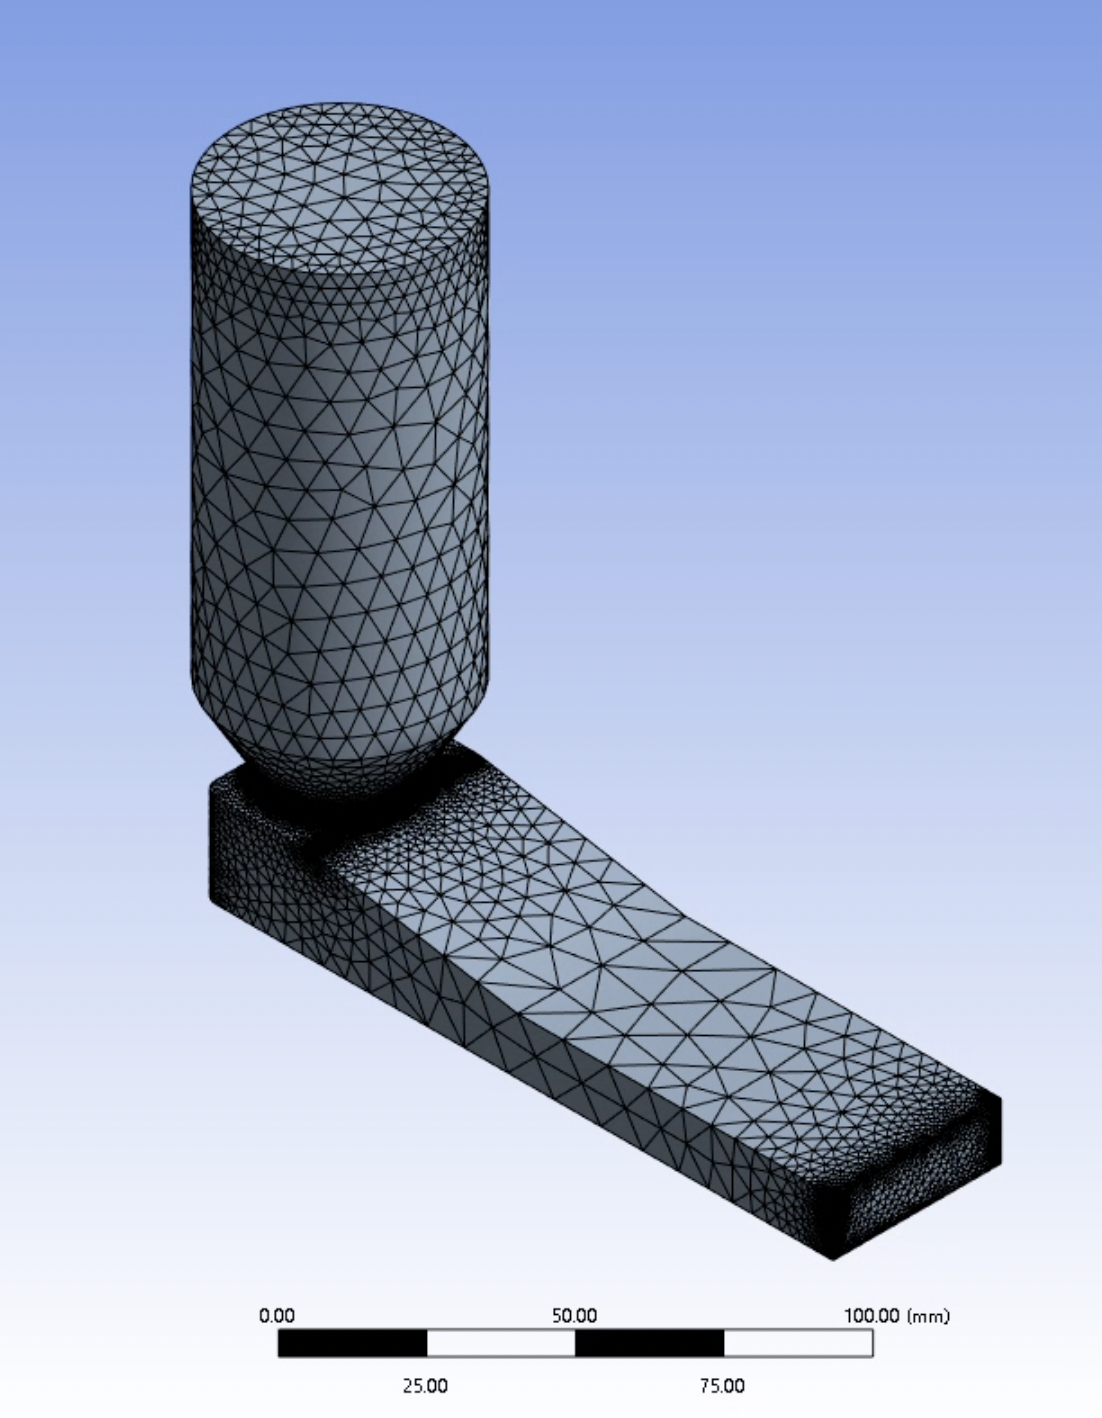
\includegraphics[width=0.7\textwidth]{figures/2.5.png}
  \caption{整体网格示意图（Baseline工况）}
  \label{fig:2.5}
\end{figure}

\begin{figure}[!htb]
  \centering
  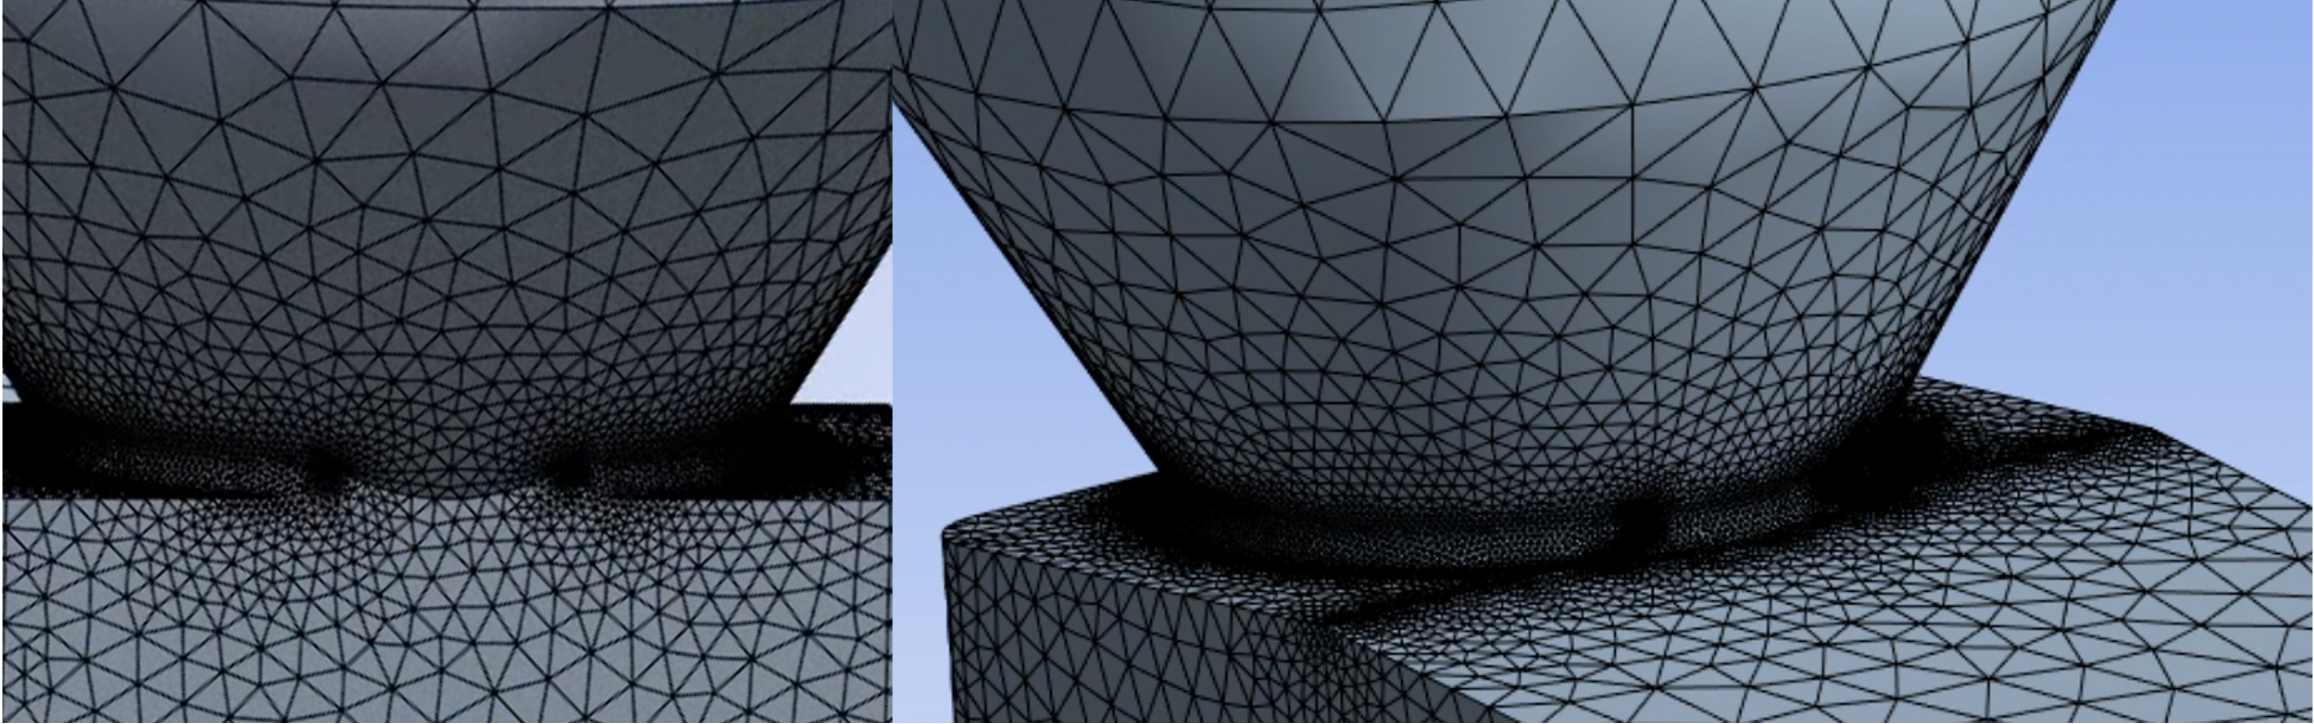
\includegraphics[width=0.7\textwidth]{figures/2.6.png}
  \caption{喷嘴收缩段与整形板受限区局部加密细节图}
  \label{fig:2.6}
\end{figure}

\subsection{网格质量评估}

\cref{tab:2.3}列出了代表性工况的网格质量评价结果。各工况网格均满足CFD数值计算对网格质量的基本要求，能够保证求解过程的稳定性与计算结果的可靠性。

针对NSGA-II优化验证工况（见\cref{chap:optimization}第\ref{sec:nsga2}节），进一步对网格切向偏斜度（Tangent Skewness）进行了检查，其最大值为3.25，仍处于可接受范围内，表明网格质量能够满足复杂流场条件下的数值模拟需求。

\begin{table}[!htb]
  \centering
  \caption{各代表性工况网格质量汇总}\label{tab:2.3}
  \renewcommand{\arraystretch}{1.3}
  \begin{tabular}{cccccp{2.5cm}}
    \toprule
    \textbf{工况} & \textbf{最大面面积} & \textbf{最小单元体积} & \textbf{最小正交性质量} & \textbf{最大长宽比} & \textbf{备注} \\
    \midrule
    Baseline       & 7.77E-05 & 6.12E-14 & 0.202 & 14.92 & 代表性工况 \\
    A1-4           & 1.37E-04 & 8.15E-14 & 0.177 & 17.03 & 收缩段最大 \\
    C3             & 1.18E-04 & 9.53E-15 & 0.204 & 16.29 & 最优工况 \\
    Pareto Optimum & 2.16E-04 & 2.98E-14 & 0.202 & 16.63 & Skewness=3.25 \\
    \bottomrule
  \end{tabular}
  \vspace{0.5em}
  
  \footnotesize{*其余工况均满足Min Orth.Q $>0.17$, Max AR $<18$。}
\end{table}

\subsection{网格无关性验证}

为评估数值结果对网格密度的敏感性并确定满足精度要求的最优网格方案，本文以C3工况（$\theta = 60°$，$L = 20$~mm，$TL = 60$~mm，$\alpha = 15°$，含边角圆滑处理）为验证对象，系统开展网格无关性研究。C3工况几何复杂度最高（含喷嘴收缩段、整形板倾斜面与圆角过渡区），对网格质量的要求最为严苛，将其作为验证工况具有代表性，可覆盖本研究全部工况。

网格无关性验证选取基底面（Substrate）的面积加权平均静压力$P_{sub,AWA}$作为网格无关性监测量。该指标为本研究的核心评价目标，对流场细节（尤其是整形板约束区近壁速度梯度与压力分布）最为敏感，适合作为网格收敛性的判别基准。

实验共设置五组全局网格尺寸：12.9~mm（粗）、8~mm、5~mm、3~mm和1~mm，在保持边界层Inflation设置（5层，增长比1.2）和关键区域局部加密策略不变的前提下，仅系统改变全局网格尺寸。各组网格统计数据与监测量结果汇总于\cref{tab:2.4}。

\begin{table}[!htb]
  \centering
  \caption{网格无关性验证数据（C3工况）}\label{tab:2.4}
  \renewcommand{\arraystretch}{1.3}
  \begin{tabular}{ccccl}
    \toprule
    \textbf{网格尺寸} & \textbf{最大长宽比} & $P_{sub,AWA}$ \textbf{(Pa)} & \textbf{与3 mm误差(\%)} & \textbf{评级} \\
    \midrule
    12.9 mm（粗）     & 16.2866 & 21702 & 2.5\% & 粗网格，通过 \\
    8 mm              & 17.3505 & 21503 & 3.5\% & 合格 \\
    5 mm              & 16.5882 & 22090 & 0.8\% & 推荐网格 \\
    3 mm（基准）       & 15.4398 & 22273 & ---    & 参考基准 \\
    1 mm              & 17.9311 & 22579 & 1.4\% & 曲面振荡，不采用 \\
    \bottomrule
  \end{tabular}
\end{table}

收敛性分析结果如\cref{fig:2.7}所示。

\begin{figure}[!htb]
  \centering
  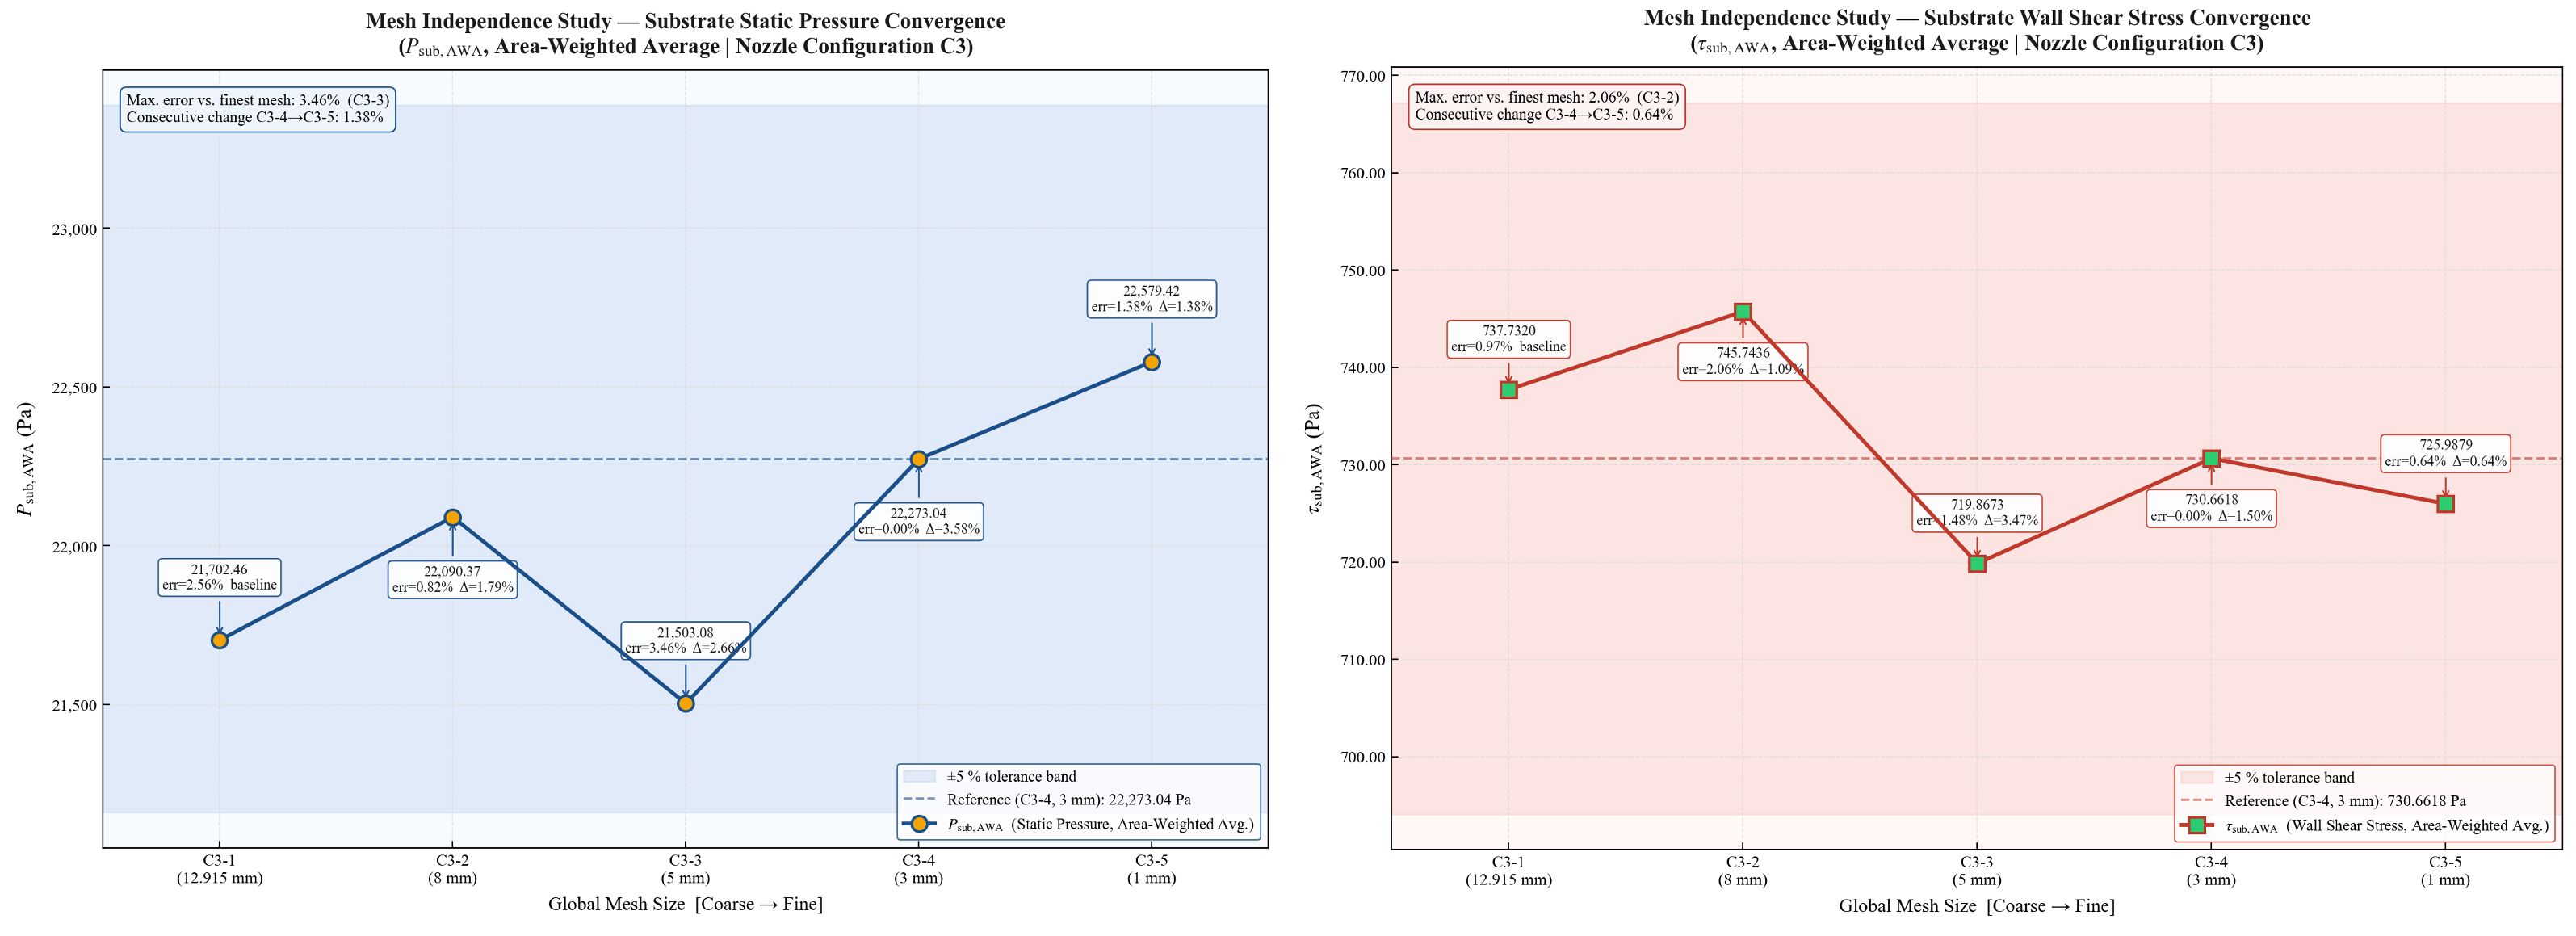
\includegraphics[width=0.9\textwidth]{figures/2.7.png}
  \caption{网格无关性验证收敛曲线（左：$P_{sub,AWA}$，右：$WSS_{nozzle}$）}
  \label{fig:2.7}
\end{figure}

以3~mm网格结果作为基准参考值，定义相对误差为：
\begin{equation}\label{eq:mesh-err}
  \varepsilon_{mesh} = \frac{|P_{sub,AWA}^{(N)} - P_{sub,AWA}^{(3mm)}|}{P_{sub,AWA}^{(3mm)}} \times 100\%.
\end{equation}
结果表明，从12.9~mm到8~mm网格，$P_{sub,AWA}$由21702~Pa降至21503~Pa，相对误差为3.5\%；从8~mm细化至5~mm时，误差降至0.8\%，已满足本研究设定的5\%收敛准则；从5~mm进一步细化至3~mm，误差仅为0.8\%，结果趋于稳定，网格无关性得到充分验证。

另外，1~mm网格虽然单元数量最多，但$P_{sub,AWA}$反而偏低（22579~Pa），且入口压力出现异常波动，偏离收敛趋势。这可能是由于在fillet曲面区域，1~mm全局网格尺寸与局部曲率不匹配，产生了高度畸变的楔形单元（最小体积达$7.9 \times 10^{-15}$~m³），诱发数值振荡。因此，1mm网格结果不纳入收敛判断。该现象同时说明：对于含曲面几何的问题，一味加密全局网格并不必然改善精度，有可能会产生截然相反的效果。针对有限元分析问题，合理的局部加密策略有时更为关键。

综合考虑计算精度与计算效率，本研究选定5~mm为推荐全局网格尺寸。在该网格方案下，$P_{sub,AWA}$与3~mm基准值的误差仅为0.8\%，远低于5\%的验收标准，同时计算时间相较3~mm方案减少约60\%，具有良好的工程实用性。本研究其余19个参数化工况均采用与C3验证工况相同的网格策略（5~mm全局尺寸、收缩段及近壁区局部加密），以确保各工况间结果的可比性。

\section{边界条件与求解设置}

\subsection{边界条件}

流体计算域入口采用速度入口边界条件，混凝土浆体速度矢量与入口截面法向一致并沿竖直向下方向施加，速度大小设定为0.03~m/s，用于表征稳定挤出工况下的进料过程；延伸段出口采用压力出口边界条件，静压设为0~Pa（表压），以模拟外界大气环境并减弱出口回压对内部流场的影响；其余所有固体边界，包括喷嘴内壁、整形板壁面以及基底接触面，均统一设置为无滑移壁面条件（No-slip），壁面速度为零，用于反映混凝土浆体与固体界面间的黏附与剪切效应；同时在整个计算域中施加重力作用，方向沿Y轴负向，与前述坐标系定义一致；上述边界条件与重力设定参数统一汇总于\cref{tab:2.5}。

\begin{table}[!htb]
  \centering
  \caption{边界条件汇总}\label{tab:2.5}
  \renewcommand{\arraystretch}{1.3}
  \begin{tabular}{lllp{4.5cm}}
    \toprule
    \textbf{边界面} & \textbf{类型} & \textbf{数值设定} & \textbf{物理说明} \\
    \midrule
    velocity\_inlet   & Velocity Inlet  & $v = 0.03$ m/s        & 泵送挤出速度，法向入射 \\
    pressure\_outlet  & Pressure Outlet & 0 Pa（表压）          & 延伸段末端自由出口 \\
    wall\_nozzle      & Wall            & No-slip               & 喷嘴内壁（收缩段+直管段） \\
    wall\_trowel      & Wall            & No-slip               & 整形板各壁面（顶/侧/前） \\
    wall\_substrate   & Wall            & No-slip               & 基底面（接触压力提取面） \\
    重力              & Body Force      & $-9.81$ m/s²（Y轴）   & 开启以影响接触压力场 \\
    \bottomrule
  \end{tabular}
\end{table}

\subsection{求解器设置}

数值求解采用ANSYS Fluent压力基（Pressure-Based）稳态求解器，以适用于低速、高黏度的非牛顿流动问题。压力-速度耦合采用SIMPLE算法以保证迭代过程中的质量守恒与收敛稳定性。空间离散方面，梯度项采用Least Squares Cell Based方法进行计算，以提高非结构化网格条件下梯度重构的精度；压力项采用PRESTO!格式，以增强对低速流动及强压力梯度区域的数值稳定性；动量方程采用Second Order Upwind格式进行离散，以提高对对流项的计算精度并降低数值扩散误差。

为了在保证数值收敛的情况下提高计算效率，连续性方程残差及各速度分量残差均控制在$1 \times 10^{-4}$以下，以作为稳态收敛判定标准。在松弛因子设置上，为适应高黏度非牛顿流体的数值特性并提高计算稳定性，压力松弛因子取0.3，动量松弛因子取0.7。所有定义的求解器参数如\cref{tab:2.6}所示，基准工况的残差收敛曲线如\cref{fig:2.8}所示。

\begin{table}[!htb]
  \centering
  \caption{求解器参数设置汇总}\label{tab:2.6}
  \renewcommand{\arraystretch}{1.3}
  \begin{tabular}{llp{6cm}}
    \toprule
    \textbf{求解器选项} & \textbf{设定值} & \textbf{说明} \\
    \midrule
    求解器类型      & Pressure-Based       & 不可压缩稳态 \\
    湍流模型        & Laminar              & $Re_{general} \approx 0.007 \ll 1$ \\
    压力--速度耦合   & SIMPLE               & 收敛稳定 \\
    压力格式        & PRESTO!              & 低速高黏度推荐 \\
    动量格式        & Second Order Upwind  & 精度优先 \\
    收敛准则        & $<1 \times 10^{-4}$  & 连续性+速度分量 \\
    压力松弛因子    & 0.3                  & 高黏度保守取值 \\
    动量松弛因子    & 0.5                  & 高黏度保守取值 \\
    迭代步数        & 500（典型）          & 所有工况500步内收敛 \\
    \bottomrule
  \end{tabular}
\end{table}

\begin{figure}[!htb]
  \centering
  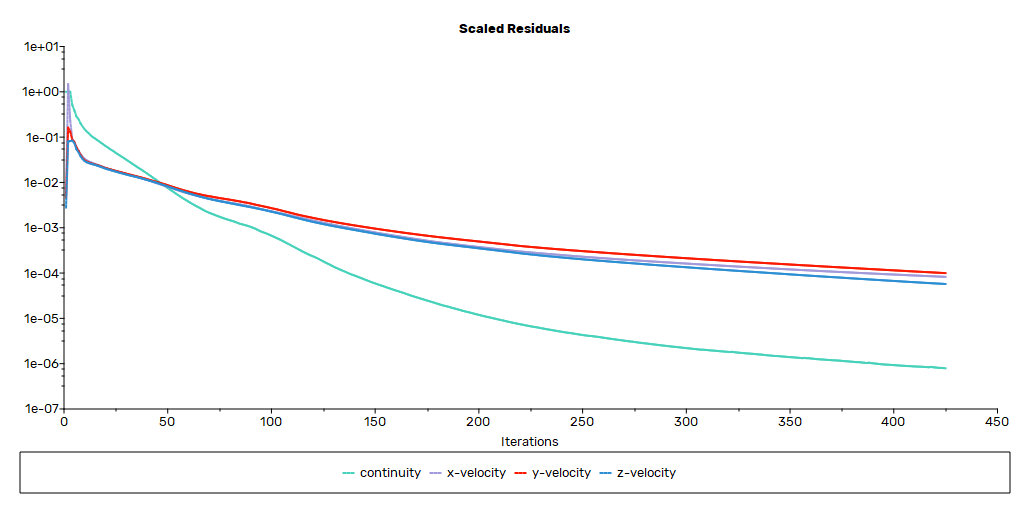
\includegraphics[width=0.8\textwidth]{figures/2.8.png}
  \caption{典型工况残差收敛曲线（Baseline工况）}
  \label{fig:2.8}
\end{figure}

\subsection{质量守恒验证}

为检验数值求解结果的稳定性与物理一致性，在ANSYS Fluent求解过程中对喷嘴入口与延伸段出口的质量流率进行监测，并记录两者差值的绝对值随迭代步数的变化曲线，用以评估质量守恒误差及收敛行为。

结果表明，所有工况在初始迭代阶段（约前50步）存在一定幅度的数值波动，随后差值逐渐衰减并趋于稳定，最终稳定在接近0的水平，说明系统在稳态求解过程中已满足质量守恒条件。由此可认为，各工况计算结果均已达到收敛状态，且数值求解具有良好的稳定性与物理合理性。基础工况的质量流率差值曲线如\cref{fig:2.9}所示。

\begin{figure}[!htb]
  \centering
  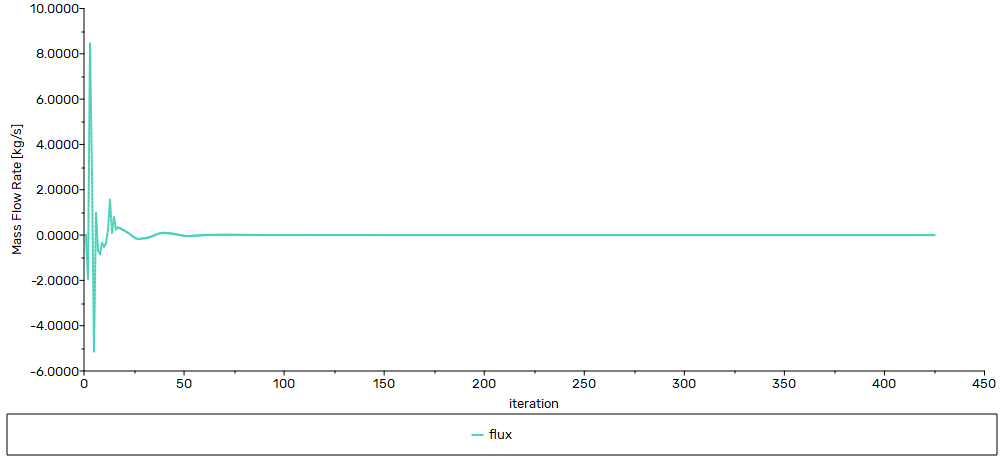
\includegraphics[width=0.8\textwidth]{figures/2.9.png}
  \caption{典型工况质量流率差值曲线（Baseline工况）}
  \label{fig:2.9}
\end{figure}
